\subsection{Instrumentation Amplifier}

	In general, sensors and tranducers have very low voltage output levels (specially passive transducers), and therefore an amplification is fundamental. The most commonly used amplifier circuit in instrumentation engineering is the common joint differential amplifier more commonly refered as \textit{Instrumentation Amplifier} (Figure \ref{fig-instrumentation-amplifier}), which is very stable and significantly reduces the output signal noise \cite{wait1975introduction}.

		\begin{figure}[htbp]
			\centering
				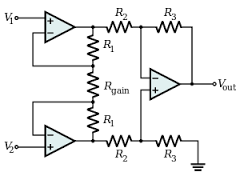
\includegraphics[scale=1.1]{figuras/fig-instrumentation-amp.png}
			\caption{Instrumentation Amplifier \cite{3opamp}}
			\label{fig-instrumentation-amplifier}
		\end{figure}


